\documentclass[12pt, a4paper]{extarticle}
\usepackage{GOST}
\usepackage{array}
\usepackage{verbatim}
\usepackage[detect-all]{siunitx}
\usepackage{amsmath}
\usepackage{amssymb}
\usepackage[utf8]{inputenc}
\usepackage{hyperref}
\usepackage{tempora}

\makeatletter
\renewcommand\@biblabel[1]{#1.}
\makeatother

\usepackage{listings}
\lstset{ 
	language=Prolog,
	basicstyle=\small, 
	numbers=left, 
	numberstyle=\tiny,
	stepnumber=1,
	numbersep=5pt,
	showspaces=false,            
	showstringspaces=false,      
	showtabs=false,             
	frame=single,            % рисовать рамку вокруг кода
	tabsize=4,      
	commentstyle=\color{green},
	keywordstyle=\color{blue}\textbf,
	numberstyle=\scriptsize\color{gray}, % the style that is used for the line-numbers
	rulecolor=\color{black},
	captionpos=t,
	breaklines=true,         % автоматически переносить строки 
	breakatwhitespace=false, % переносить строки по пробелу
	%escapeinside={\#*}{*)} 
}



\begin{document}
	
\begin{table}[ht]
	\centering
	\begin{tabular}{|c|p{400pt}|} 
		\hline
		\begin{tabular}[c]{@{}c@{}} 
\includegraphics[scale=1]{source/b_logo.jpg} \\\end{tabular} &
		\footnotesize\begin{tabular}[c]{@{}c@{}}\textbf{Министерство~науки~и~высшего~образования~Российской~Федерации}\\\textbf{Федеральное~государственное~бюджетное~образовательное~учреждение}\\\textbf{~высшего~образования}\\\textbf{«Московский~государственный~технический~университет}\\\textbf{имени~Н.Э.~Баумана}\\\textbf{(национальный~исследовательский~университет)»}\\\textbf{(МГТУ~им.~Н.Э.~Баумана)}\\\end{tabular}  \\
		\hline
	\end{tabular}
\end{table}
\noindent\rule{\textwidth}{4pt}
\noindent\rule[14pt]{\textwidth}{1pt}
\hfill 
\noindent
\makebox{ФАКУЛЬТЕТ~}%
\makebox[\textwidth][l]{\underline{~«Информатика и системы управления»~~~~~~~~~~~~~~~~~~~~~~~~~~~~~~~~~}}%
\\
\noindent
\makebox{КАФЕДРА~}%
\makebox[\textwidth][l]{\underline{~«Программное обеспечение ЭВМ и информационные технологии»~}}%
\\

\begin{center}
	\vspace{1.5cm}
	{\bf\huge Отчёт\par}
	{\bf\Large по лабораторной работе № 13\par}
	\vspace{0.7cm}
\end{center}


\noindent
\makebox{\large{\bf Название:}~~~}
\makebox[\textwidth][l]{\large\underline{~Работа программы на Prolog~}}\\

\noindent
\makebox{\large{\bf Дисциплина:}~~~}
\makebox[\textwidth][l]{\large\underline{~Функциональное и логическое программирование~}}\\

\vspace{1.5cm}
\noindent
\begin{tabular}{l c c c c c}
	Студент      & ~ИУ7-65Б~               & \hspace{2.5cm} & \hspace{2cm}                 & &  Д.В. Сусликов \\\cline{2-2}\cline{4-4} \cline{6-6} 
	\hspace{3cm} & {\footnotesize(Группа)} &                & {\footnotesize(Подпись, дата)} & & {\footnotesize(И.О. Фамилия)}
\end{tabular}

\noindent
\begin{tabular}{l c c c c}
	Преподаватель & \hspace{5cm}   & \hspace{2cm}                 & & ~~~~~~Н.Б. Толпинская~~~~~~\\\cline{3-3} \cline{5-5} 
	\hspace{3cm}  &                & {\footnotesize(Подпись, дата)} & & {\footnotesize(И.О. Фамилия)}
\end{tabular}

\vspace{0.6cm}
\begin{center}	
	\vfill
	\large \textit {Москва, 2021}
\end{center}

\thispagestyle {empty}
\pagebreak

\clearpage


\textbf{Цель работы} - получить навыки построения модели предметной областиб разработки и оформления программы на Prolog, изучить принципы, логику формирования программы и отдельные шаги выполнения программы на Prolog.

\textbf{Задание}

Составить программу, т.е. модель предметной области – базу знаний, объединив в ней информацию – знания:

\begin{enumerate}
	\item \textbf{<<Телефонный справочник>>}: Фамилия, №тел, Адрес – структура (Город, Улица, №дома, №кв),
	\item \textbf{<<Автомобили>>}: Фамилия\_владельца, Марка, Цвет, Стоимость, и др.,
	\item \textbf{<<Вкладчики банков>>}: Фамилия, Банк, счет, сумма, др.
\end{enumerate}

Владелец может иметь несколько телефонов, автомобилей, вкладов (Факты).

\hfill

Используя правила, обеспечить возможность поиска:

\begin{enumerate}
	\item 
	\begin{enumerate}
		\item По № телефона найти: Фамилию, Марку автомобиля, Стоимость автомобиля (может быть несколько),
		\item Используя сформированное в пункте а) правило, по № телефона найти: только Марку автомобиля (автомобилей может быть несколько),
	\end{enumerate}
	\item Используя простой, не составной вопрос: по Фамилии (уникальна в городе, но в разных городах есть однофамильцы) и Городу проживания найти:  Улицу проживания, Банки, в которых есть вклады и №телефона. 
\end{enumerate}

\textbf{Для задания1 и задания2: }

для одного из вариантов ответов, и для а) и для в), описать словесно порядок поиска ответа на вопрос, указав, как выбираются знания, и, при этом, для каждого этапа унификации, выписать подстановку – наибольший общий унификатор, и соответствующие примеры термов.


\newpage
\textbf{Листинг:}
\begin{lstlisting}
	domains
		number, surname, city, street, brand, color, bank = symbol.
		building_num, room_num, price, bill, summa = integer.
		address = address(city, street, building_num, room_num).	
	predicates
		phonebook(surname, number, address).
		car(surname, brand, color, price).
		depositor(surname, bank, bill, summa).
		find_by_phone(number, surname, brand, price).
		brand_by_phone(number, brand).
		info_by_surname_and_city(surname, city, street, bank, number).
	clauses
		phonebook("Surname1", "11111", address("City1", "St.1", 1, 17)).
		phonebook("Surname2", "22222", address("City2", "St.2", 2, 18)).
		phonebook("Surname3", "33333", address("City1", "St.1", 4, 28)).
		phonebook("Surname4", "11111", address("City3", "St.4", 4, 24)).
		
		car("Surname1", "Brand1", "Red", 12345).
		car("Surname1", "Brand2", "Blue", 3000).
		car("Surname2", "Brand1", "Black", 2000).
		
		depositor("Surname1", "Bank1", 3221, 1200).
		depositor("Surname1", "Bank2", 1233, 4000).
		depositor("Surname2", "Bank2", 4356, 2000).	
		
		find_by_phone(Number, Surname, Brand, Price):- phonebook(Surname, Number, _), car(Surname, Brand, _, Price).
		brand_by_phone(Number, Brand):- find_by_phone(Number, _, Brand, _).
		info_by_surname_and_city(Surname, City, Street, Bank, Number):- phonebook(Surname, Number, address(City, Street, _, _)),
		depositor(Surname, Bank, _, _).
	goal
		%find_by_phone("11111", Surname, Brand, Price).
		%find_by_phone("22222", Surname, Brand, Price).
		%find_by_phone("12345", Surname, Brand, Price).
		
		%brand_by_phone("11111", Brand).
		%brand_by_phone("22222", Brand).
		%brand_by_phone("12345", Brand).
		
		%info_by_surname_and_city("Surname1", "City1", Street, Bank, Number).
		%info_by_surname_and_city("Surname2", "City2", Street, Bank, Number).
		%info_by_surname_and_city("Surname4", "City17", Street, Bank, Number).
\end{lstlisting}

\newpage
\textbf{Результат работы:}\par

\textbf{Задание 1a} \par
\begin{figure}[h!]	
	\center{
\includegraphics{source/1.1.png} \\ Пример 1}	
\end{figure}\par

\begin{figure}[h!]	
	\center{
\includegraphics{source/1.2.png} \\ Пример 2}	
\end{figure}\par

\begin{figure}[h!]	
	\center{
\includegraphics{source/no_sol.png} \\ Пример 3}	
\end{figure}\par

\newpage
Разбор "Примера 1" find\_by\_phone("11111", Surname, Mark, Price). \par 
\begin{table}[h!]
	\begin{tabular}{|l|l|l|}
		\hline
		Шаг & Сравнимые термы; результаты; подстановка, если есть                                                                                                                                                                                                                   & Дальнейшие действия                                                                                                                       \\ \hline
		0   & \begin{tabular}[c]{@{}l@{}}find\_by\_phone("11111", Surname, Brand, Price) = \\ phonebook("Surname1", "11111", address("City1", "St.1", 1, 17)).\\ Разные функторы. Унификация не успешна.\end{tabular}                                                               & \begin{tabular}[c]{@{}l@{}}Переход к следующему\\ предложению\end{tabular}                                                                \\ \hline
		& ...                                                                                                                                                                                                                                                                   &                                                                                                                                           \\ \hline
		4   & \begin{tabular}[c]{@{}l@{}}find\_by\_phone("11111", Surname, Brand, Price) =\\ car("Surname1", "Brand1", "Red", 12345).\\ Разные функторы. Унификация не успешна.\end{tabular}                                                                                        & \begin{tabular}[c]{@{}l@{}}Переход к следующему\\ предложению\end{tabular}                                                                \\ \hline
		& ...                                                                                                                                                                                                                                                                   &                                                                                                                                           \\ \hline
		7   & \begin{tabular}[c]{@{}l@{}}find\_by\_phone("11111", Surname, Brand, Price) =\\ depositor("Surname1", "Bank1", 3221, 1200).\\ Разные функторы. Унификация не успешна.\end{tabular}                                                                                     & \begin{tabular}[c]{@{}l@{}}Переход к следующему\\ предложению\end{tabular}                                                                \\ \hline
		& ...                                                                                                                                                                                                                                                                   &                                                                                                                                           \\ \hline
		10  & \begin{tabular}[c]{@{}l@{}}find\_by\_phone("11111", Surname, Brand, Price) =\\ find\_by\_phone(Number, Surname, Brand, Price).\\ Унификация успешна.\\ $\theta$ = \{Number = "11111", Surname = Surname,\\ Brand = Brand, Price = Price\}\end{tabular}   & \begin{tabular}[c]{@{}l@{}}Новое состояние\\ резольвенты:\\ phonebook(Surname, Number, \_)\\ car(Surname, Brand, \_, Price).\end{tabular} \\ \hline
		11  & \begin{tabular}[c]{@{}l@{}}phonebook(Surname, 11111, \_) =\\ phonebook("Surname1", "11111", address("City1", "St.1", 1, 17)).\\ Унификация успешна.\\ $\theta$ = \{Number = "11111", Surname = "Surname1",\\ Brand = Brand, Price = Price\}\end{tabular} & \begin{tabular}[c]{@{}l@{}}Новое состояние\\ резольвенты:\\ car(Surname, Brand, \_, Price).\end{tabular}                                  \\ \hline
		12  & \begin{tabular}[c]{@{}l@{}}car("Surname1", Brand, \_, Price) =\\ phonebook("Surname1", "11111", address("City1", "St.1", 1, 17)).\\ Разные функторы. Унификация не успешна.\end{tabular}                                                                              & \begin{tabular}[c]{@{}l@{}}Переход к следующему\\ предложению\end{tabular}                                                                \\ \hline
		& ...                                                                                                                                                                                                                                                                   &                                                                                                                                           \\ \hline
		16  & \begin{tabular}[c]{@{}l@{}}car("Surname1", Brand, \_, Price) =\\ car("Surname1", "Brand1", "Red", 12345).\\ Унификация успешна.\\ $\theta$ = \{Number = "11111", Surname = "Surname1",\\ Brand = "Brand1", Price = 12345\}\end{tabular}                  & \begin{tabular}[c]{@{}l@{}}Новое состояние \\ резольвенты: Пусто\\ Вывод:\\ Surname=Surname1, \\ Brand=Brand1, Price=12345\end{tabular}   \\ \hline
	\end{tabular}
\end{table}
\newpage

\textbf{Задание 1b} \par
\begin{figure}[h!]	
	\center{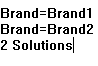
\includegraphics{source/2.1.png} \\ Пример 4}	
\end{figure}\par

\begin{figure}[h!]	
	\center{
\includegraphics{source/2.2.png} \\ Пример 5}	
\end{figure}\par

\begin{figure}[h!]	
	\center{
\includegraphics{source/no_sol.png} \\ Пример 6}	
\end{figure}\par

\newpage
Разбор "Примера 4" brand\_by\_phone("11111", Brand). \par 

\begin{table}[h!]
	\begin{tabular}{|l|l|l|}
		\hline
		Шаг & Сравнимые термы; результаты; подстановка, если есть                                                                                                                                           & Дальнейшие действия                                                                                                 \\ \hline
		0   & \begin{tabular}[c]{@{}l@{}}brand\_by\_phone("11111", Brand) =\\ phonebook("Surname1", "11111", address("City1", "St.1", 1, 17))\\ Разные функторы. Унификация не успешна.\end{tabular}        & \begin{tabular}[c]{@{}l@{}}Переход к следующему\\ предложению\end{tabular}                                          \\ \hline
		& ...                                                                                                                                                                                           &                                                                                                                     \\ \hline
		4   & \begin{tabular}[c]{@{}l@{}}brand\_by\_phone("11111", Brand) =\\ car("Surname1", "Brand1", "Red", 12345).\\ Разные функторы. Унификация не успешна.\end{tabular}                               & \begin{tabular}[c]{@{}l@{}}Переход к следующему\\ предложению\end{tabular}                                          \\ \hline
		& ...                                                                                                                                                                                           &                                                                                                                     \\ \hline
		7   & \begin{tabular}[c]{@{}l@{}}brand\_by\_phone("11111", Brand) =\\ depositor("Surname1", "Bank1", 3221, 1200).\\ Разные функторы. Унификация не успешна.\end{tabular}                            & \begin{tabular}[c]{@{}l@{}}Переход к следующему\\ предложению\end{tabular}                                          \\ \hline
		& ...                                                                                                                                                                                           &                                                                                                                     \\ \hline
		10  & \begin{tabular}[c]{@{}l@{}}brand\_by\_phone("11111", Brand) =\\ find\_by\_phone(Number, Surname, Brand, Price)\\ Разные функторы. Унификация не успешна.\end{tabular}                         & \begin{tabular}[c]{@{}l@{}}Переход к следующему\\ предложению\end{tabular}                                          \\ \hline
		11  & \begin{tabular}[c]{@{}l@{}}brand\_by\_phone("11111", Brand) =\\ brand\_by\_phone(Number, Brand)\\ Унификация успешна.\\ $\theta$ = \{Number = "11111", Brand = Brand\}\end{tabular}              & \begin{tabular}[c]{@{}l@{}}Новое состояние\\ резольвенты:\\ find\_by\_phone("11111",\\  \_, Brand, \_)\end{tabular} \\ \hline
		12  & \begin{tabular}[c]{@{}l@{}}find\_by\_phone("11111", \_, Brand, \_) =\\ phonebook("Surname1", "11111", address("City1", "St.1", 1, 17))\\ Разные функторы. Унификация не успешна.\end{tabular} & \begin{tabular}[c]{@{}l@{}}Переход к следующему\\ предложению\end{tabular}                                          \\ \hline
		& ...                                                                                                                                                                                           &                                                                                                                     \\ \hline
		16  & \begin{tabular}[c]{@{}l@{}}find\_by\_phone("11111", \_, Brand, \_) =\\ car("Surname1", "Brand1", "Red", 12345).\\ Разные функторы. Унификация не успешна.\end{tabular}                        & \begin{tabular}[c]{@{}l@{}}Переход к следующему\\ предложению\end{tabular}                                          \\ \hline
		& ...                                                                                                                                                                                           &                                                                                                                     \\ \hline
		19  & \begin{tabular}[c]{@{}l@{}}find\_by\_phone("11111", \_, Brand, \_) =\\ depositor("Surname1", "Bank1", 3221, 1200).\\ Разные функторы. Унификация не успешна.\end{tabular}                     & \begin{tabular}[c]{@{}l@{}}Переход к следующему\\ предложению\end{tabular}                                          \\ \hline
		& ...                                                                                                                                                                                           &                                                                                                                     \\ \hline
	\end{tabular}
\end{table}
\newpage

\begin{table}[h!]
	\begin{tabular}{|l|l|l|}
		\hline
		22  & \begin{tabular}[c]{@{}l@{}}find\_by\_phone("11111", \_, Brand, \_) =\\ find\_by\_phone(Number, Surname, Brand, Price)\\ Унификация успешна.\\ $\theta$ = \{Number = "11111", Brand = Brand\}\end{tabular}                                   & \begin{tabular}[c]{@{}l@{}}Новое состояние\\ резольвенты:\\ phonebook(Surname,\\ "11111", \_),\\ car(Surname, Brand,\\ \_, Price).\end{tabular} \\ \hline
		23  & \begin{tabular}[c]{@{}l@{}}phonebook(Surname, "11111", \_) =\\ phonebook("Surname1", "11111", address("City1", "St.1", 1, 17)).\\ Унификация успешна.\\ $\theta$ = \{Surname = "Surname1", Number = "11111",\\ Brand = Brand\}\end{tabular} & \begin{tabular}[c]{@{}l@{}}Новое состояние\\ резольвенты:\\ car("Surname1", Brand,\\ \_, Price).\end{tabular}                                   \\ \hline
		24  & \begin{tabular}[c]{@{}l@{}}car("Surname1", Brand,\_, Price) =\\ phonebook("Surname1", "11111", address("City1", "St.1", 1, 17)).\\ Разные функторы. Унификация не успешна.\end{tabular}                                                  & \begin{tabular}[c]{@{}l@{}}Переход к следующему\\ предложению\end{tabular}                                                                      \\ \hline
		& ...                                                                                                                                                                                                                                      &                                                                                                                                                 \\ \hline
		28  & \begin{tabular}[c]{@{}l@{}}car("Surname1", Brand, \_, Price) =\\ car("Surname1", "Brand1", "Red", 12345)\\ Унификация успешна.\\ $\theta$ = \{Surname = "Surname1", Number = "11111",\\ Brand = "Brand1"\}\end{tabular}                     & \begin{tabular}[c]{@{}l@{}}Новое состояние\\ резольвенты:\\ Пусто\\ \\ Вывод:\\ Brand = Brand1\end{tabular}                                     \\ \hline
	\end{tabular}
\end{table}

\newpage
\textbf{Задание 2} \par
\begin{figure}[h!]	
	\center{
\includegraphics{source/3.1.png} \\ Пример 7}	
\end{figure}\par

\begin{figure}[h!]	
	\center{
\includegraphics{source/3.2.png} \\ Пример 8}	
\end{figure}\par

\begin{figure}[h!]	
	\center{
\includegraphics{source/no_sol.png} \\ Пример 9}	
\end{figure}\par

\newpage
Разбор "Примера 7"  info\_by\_surname\_and\_city("Surname1", "City1", Street, Bank, Number) \par 

\begin{table}[h!]
	\begin{tabular}{|l|l|l|}
		\hline
		Шаг & Сравнимые термы; результаты; подстановка, если есть                                                                                                                                                                                                                                                                   & Дальнейшие действия                                                                                                                                                                   \\ \hline
		0   & \begin{tabular}[c]{@{}l@{}}info\_by\_surname\_and\_city("Surname1", "City1", \\ Street, Bank, Number) =\\ phonebook("Surname1", "11111",\\  address("City1", "St.1", 1, 17)).\\ Разные функторы. Унификация не успешна.\end{tabular}                                                                                  & \begin{tabular}[c]{@{}l@{}}Переход к следующему\\ предложению\end{tabular}                                                                                                            \\ \hline
		& ...                                                                                                                                                                                                                                                                                                                   &                                                                                                                                                                                       \\ \hline
		12  & \begin{tabular}[c]{@{}l@{}}info\_by\_surname\_and\_city("Surname1", "City1", \\ Street, Bank, Number) =\\ info\_by\_surname\_and\_city(Surname, City, \\ Street, Bank, Number)\\ Унификация успешна.\\ $\theta$ = \{Surname = "Surname1", City = "City1",\\ Street = Street, Bank = Bank, Number = Number\}\end{tabular} & \begin{tabular}[c]{@{}l@{}}Новое состояние\\ резольвенты:\\ phonebook("Surname1", Number,\\  address("City1", Street, \_, \_)),\\ \\ depositor("Surname1", Bank, \_, \_)\end{tabular} \\ \hline
		13  & \begin{tabular}[c]{@{}l@{}}phonebook("Surname1", Number,\\  address("City1", Street, \_, \_)) =\\ phonebook("Surname1", "11111", \\  address("City1", "St.1", 1, 17))\\ Унификация успешна.\\ $\theta$ = \{Surname = "Surname1", City = "City1",\\ Street = "St.1", Bank = Bank, Number = "11111"\end{tabular}           & \begin{tabular}[c]{@{}l@{}}Новое состояние\\ резольвенты:\\ depositor("Surname1", Bank, \_, \_)\end{tabular}                                                                          \\ \hline
		14  & \begin{tabular}[c]{@{}l@{}}depositor("Surname1", Bank, \_, \_) = \\ phonebook("Surname1", "11111",\\  address("City1", "St.1", 1, 17)).\\ Разные функторы. Унификация не успешна.\end{tabular}                                                                                                                        & \begin{tabular}[c]{@{}l@{}}Переход к следующему\\ предложению\end{tabular}                                                                                                            \\ \hline
		& ...                                                                                                                                                                                                                                                                                                                   &                                                                                                                                                                                       \\ \hline
		21  & \begin{tabular}[c]{@{}l@{}}depositor("Surname1", Bank, \_, \_) =\\ depositor("Surname1", "Bank1", 3221, 1200)\\ Унификация успешна.\\ $\theta$ = \{Surname = "Surname1", City = "City1",\\ Street = "St.1", Bank = "Bank1", Number = "11111"\end{tabular}                                                                & \begin{tabular}[c]{@{}l@{}}Новое состояние\\ резольвенты:\\ Пусто\\  Вывод:\\ Street=St.1, Bank=Bank1,\\  Number=11111\end{tabular}                                                 \\ \hline
	\end{tabular}
\end{table}

\newpage
\textbf{Ответы на вопросы}\par
\begin{enumerate}
	\item Что такое терм?\\
	Терм — это основной элемнт языка в Prolog. Термы могут быть константами, переменными или составными термами. Константы могут быть числовыми, символьными атомами или строками. Переменные могут быть именованными или анонимными. Составные термы используются для обозначения отношений между объектами, они объединяют отдельные элементы знаний в единый объект.
	\item Что такое предикат в матлогике (математике)?\\
	Предикат в матлогике — это функция, которая возвращает или  0 («ложь»), или 1 («истина»).
	\item Что описывает предикат в Prolog?\\
	В Prolog предикат - отношение, определяемое процедурой(совокупностью правил, описывающих определенные отношения). 
	\item Назовите виды предложений в программе и приведите примеры таких предложений из Вашей программы. Какие предложения являются основными, а какие – не основными? Каковы: синтаксис и семантика (формальный смысл) этих предложений (основных и неосновных)?\\
	Виды предложений:
	\begin{itemize}
		\item Факты - это частный случай правила. Факт - это предложение, в котором отсутсвует тело.\\
		car("Surname1", "Brand1", "Red", 12345).
		\item Правила - обобщенная запись знаний и условий, при которых знание является истиной. Правило состоит из заголвка и тела.\\
		find\_by\_phone(Number, Surname, Brand, Price):- phonebook(Surname, Number, \_), car(Surname, Brand, \_, Price).
		\item Вопросы — используются для того, чтобы узнать истинно ли введеное предложение\\
		brand\_by\_phone("11111", Brand).
	\end{itemize}
	Основные предложения — это предложения, которые не содержат переменных.\\ Неосновные предложения — это предложения, которые содержат переменные в момент фиксации программы. \\
	Переменные пишутся с  заглавной буквы. 
	\item Каковы назначение, виды и особенности использования переменных в программе на Prolog? Какое предложение БЗ сформулировано в более общей – абстрактной форме: содержащее или не содержащее переменных?\\
	Переменные нужны для передачи знаний. Переменные могут быть именованные и анонимные. Если переменная не имеет значения, то она называется не связанной, иначе — связанной. \\
	Анонимные переменные не могут быть связаны со значением. Анонимные переменные используются в случаях, когда необходимо использовать переменную, однако ее значение не требуется.  \\
	Именованные переменные уникальны в рамках одного предложения, т.е. в разных предложениях одно и то же имя переменной может использоваться для обозначения разных объектов.\\
	Анонимные переменные уникальны везде.Все переменные безтиповые, в процессе вычисления они могут связываться с любыми объектами. \\
	Предложение содержащее переменные сформулировано в более общей-абстрактной форме, так как несколько знаний могут подойти под одно предложение. 
	\item Что такое подстановка?\\
	Подстановка - множество пар вида {Xi= ti}, где Xi–переменная, а ti–терм.
	\item Что такое пример терма? Как и когда строится? Как Вы думаете, система строит и хранит примеры?\\
	Пример терма  А — это терм B такой, что существует такая подстановка $\omega$, чтоB = A$\omega$.\\
	Примеры термов строятся в процессе унификации, когда  происходит сравнение двух термов,с помощью подстановки всех возможных значений из базы знаний. \\
	Пример хранится в памяти для продолжения доказательства. Он стирается, когда система проходит все возможные варианты, или когда на вопрос можно дать ответ «да».
\end{enumerate}
\end{document}